%%%%%%%%%%%%%%%%%%%%%%%%%%%%%%%%%%%
\chapter{Evolução do \textit{CoScore}}\label{apendice:evolucao_pontuacao_nucleo}
%%%%%%%%%%%%%%%%%%%%%%%%%%%%%%%%%%%

\begin{figure}[!htb]
  \begin{center}
    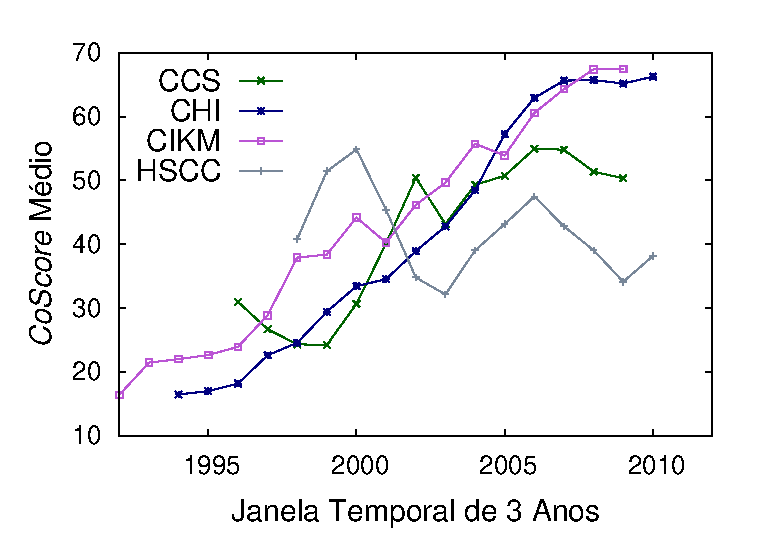
\includegraphics[scale=.6]{../graficos/average_core_score/pt_BR/average_core_score_slide_window_grupo_3_temporal_web.eps}
    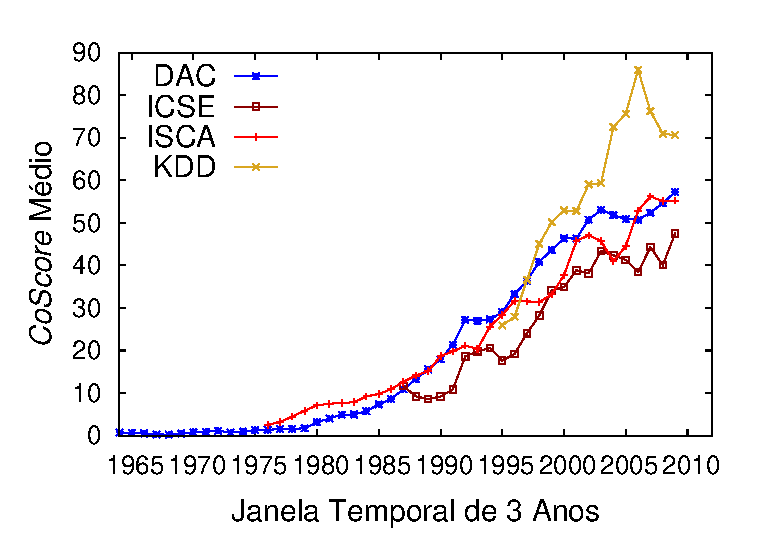
\includegraphics[scale=.6]{../graficos/average_core_score/pt_BR/average_core_score_slide_window_grupo_4_temporal_web.eps}
    \\
    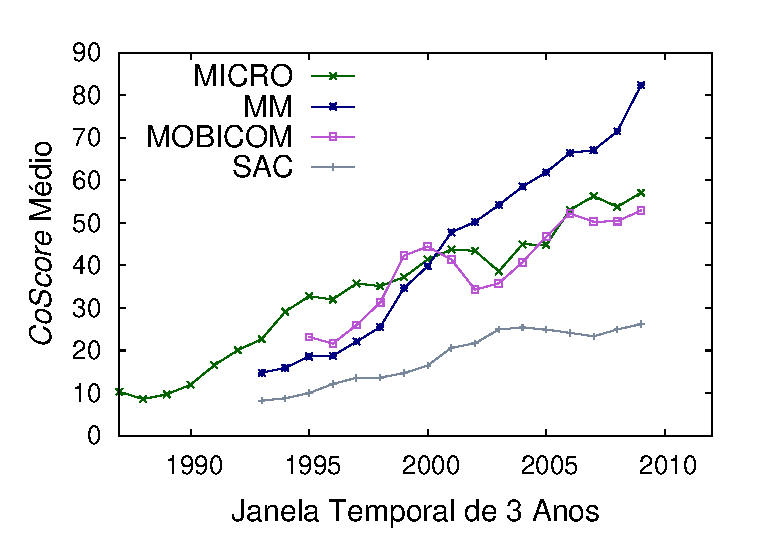
\includegraphics[scale=.6]{../graficos/average_core_score/pt_BR/average_core_score_slide_window_grupo_5_temporal_web.eps}
    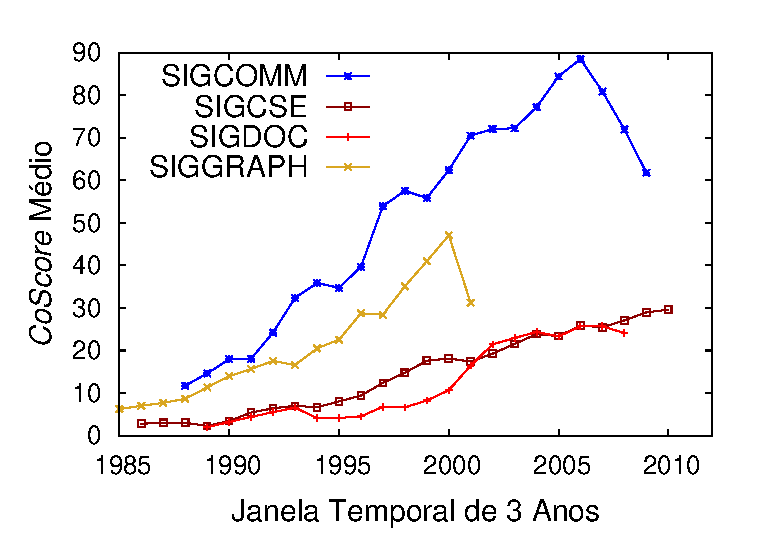
\includegraphics[scale=.6]{../graficos/average_core_score/pt_BR/average_core_score_slide_window_grupo_6_temporal_web.eps}
  \end{center}
  \caption{\textit{CoScore} médio das comunidades científicas}
  \label{fig:average_core_score_apendice}
\end{figure}